% !TEX encoding = UTF-8
% !TEX TS-program = pdflatex
% !TEX root = ../tesi.tex
% !TEX spellcheck = it-IT

%**************************************************************
\chapter{Conclusioni}
\label{cap:conclusioni}
%**************************************************************
Al di là del formalismo informatico, lo scopo principale di questo progetto era indagare sul possibile uso della tecnologia \emph{Tango} nel campo ispettivo come effettivo supporto allo studio di beni materiali. Il prototipo realizzato sembra confermare che cioè è possibile.\\
I risultati ottenuti sono stati piuttosto soddisfacenti e con qualche raffinamento appare possibile inserire l'applicazione in un contesto produttivo.

\section{Prove pratiche}
Il prototipo prodotto è stato testato in numerori ambienti e su diversi oggetti. Nella quasi totalià dei casi i risultati sono stati più che sufficienti per quanto riguarda la qualità del \emph{Point Cloud} ricostruito.\\
Per quanto riguarda invece il calcolo del volume i risultati non sono ancora totalmente sufficienti: il volume ottenuto è sempre dello stesso ordine di grandezza del volume reale, ma spesso è affetto da un errore relativo tra il 30 ed il 50\% ed un errore del genere non è affatto tollerabile. Tale divario però è facilmente appianabile migliorando la qualità delle elaborazioni dei \emph{Point Cloud} e delle \emph{mesh} lato \emph{Server}.

\section{Sviluppi futuri}
Il progetto è nato molto recentemente, dopo circa due mesi di sviluppo è stato prodotto un prototipo soddisfacente. Molti dei problemi riscostranti durante il percorso di \emph{stage} sono stati risolti, grazie ai prototipi e alle prove pratiche sono state molteplici anche le idee per rendere l'applicazione ancora più completa. Riporto qui solo alcune di queste.

\subsection{ICP su tablet}
Uno più gravi problemi delle ricostruzioni 3D effettuate tramite sovrapposizione di \emph{Point Cloud} è il \emph{ghosting}. Si tratta dello sdoppiamento di alcune "facce" dell'oggetto ricostruito.\\
\begin{figure}[!h] 
    \centering 
    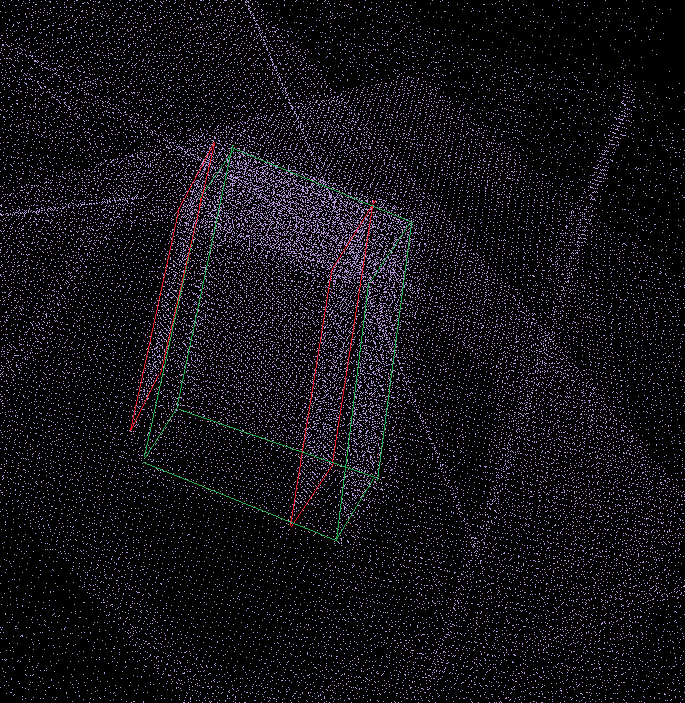
\includegraphics[width=0.9\columnwidth]{pointClouds/ghosting.png} 
    \caption{Point Cloud che presenta problemi di \emph{ghosting} di una scatola rettangolare}
    \label{figure:pcloud_ghosting}
\end{figure}
Nell'esempio in figura \ref{figure:pcloud_ghosting} sono stati evidenziati in verde gli spigoli corretti di una scatola rettangolare, mentre con colore rosso quelli dovuti al \emph{ghosting}; si può chiaramente notare che le facce laterali appaiosno sdoppiate e ciò può portare a significativi errori nella ricostruzione dell'oggetto e soprattutto nel calcolo del volume.\\
Questo fenomeno è dovuto ad errori di stima nella posizione del dispositivo, e per quanto si cerchi di ridurli essi rimarranno sempre. Si tratta di un altro limite fisico dei dispositivi \emph{Tango}, che in questo caso è aggirabile.\\
\emph{ICP} o \emph{Iterative Closest Point} è un algoritmo che cerca di minimizzare le differenze tra due nuvole di punti. Applicando \emph{ICP} su due \emph{Point Cloud} che non si sovrappongono perfettamente permetterebbe di ottenere una matrice di trasformazione da appliccare ad uno dei due per farlo combaciare all'altro. L'algoritmo in questione ha molte implentazioni in \emph{C++}, tra cui una presente proprio all'interno della libreria \emph{PCD} utilizzata lato \emph{Server}. Questo fatto ha dato modo di testare la sua effettiva efficacia.\\
Il problema è che spedire ogni singola ripresa al \emph{Server} ed aspettare una risposta sembra una strada non percorribile: per una rilevazione intera servono più di 20 riprese, senza connessione internet il servizio non sarebbe disponibile etc.\\
Per questo un possibile sviluppo futuro potrebbe essere quello di implementare \emph{ICP} lato \emph{tablet}. Ci sarebbe due vie percorribili: importare una delle tante implementazioni in \emph{C++} ed accedervi dal codice \emph{Java} mediate \emph{JNI} oppure implementare da capo l'algoritmo nativamente in \emph{Java}. Entrambe le ipotesi vanno attentamente valutate tenendo conto anche della potenza di calcolo e del consumo di batteria del dispositivo.

\subsection{Integraione C++/Jni lato tablet}
\emph{Google} fornisce oltre a delle ricche librerie \emph{Java} anche delle \emph{API} in linguaggio \emph{C/C++}. Alcune funzioni esposte da queste ultime non sono presenti in quelle \emph{Java} oppure sono molto più efficienti. Sarebbe quindi necessario, negli sviluppi futuri, predisporre una interfaccia \emph{Jni} in maniera da integrare codice \emph{Java} e \emph{C++} all'interno della stessa applicazione.\\
Tutto il progetto ne gioverebbe, specialmente per quanto riguarda le performance; inoltre si potrebbe pensare di importare parti della libreria \emph{PCD} in maniera da automatizzare alcuni processi.

\subsection{Texture dei punti}
Il prodotto fornisce delle buone ricostruzioni 3D per quanto riguarda la forma e le dimensioni dell'oggetto; ai fini ispettivi, di fatto, non c'è biosgno d'altro. Ciononostante le ricostruzioni visualizzate sia su \emph{tablet} che su \emph{computer} essendo formate da soli punti sono spesso di difficile comprensione da parte dell'utenza. Per rispondere a queste esigenza potrebbe essere opportuno pensare ad aggiungere ad ogni singolo punto una opportuna texture in maniera da rendere più immediato il riconoscimento dell'oggetto da parte dell'utente.\\
Questo sviluppo darebbe un grosso valore aggiunto in quando migliora grandemente l'aspetto grafico del sistema e lo rende quindi anche più vendibile.\\
Alcuni esempi di \emph{Point Cloud} \emph{texturizzati} sono già presenti in rete sotto licenza \emph{Open Source}, quindi è possibile pensare al riuso degli stessi.

\subsection{Rimozione artefatti}
Un altro problema che affligge le ricostruzioni 3D effettuate da \emph{Samba} è il rumore causato da forti fonti di luce o superfici riflettenti.\\
In molte riprese infatti appaiono dei piani sospesi a mezz'aria che si sommmano li uni agli altri rendendo qualche volta la ricostruzione praticamente inutilizzabile. Lato \emph{Server} essi sono spesso eliminabili dalla libreria \emph{PCD}, ma lato \emph{tablet} rendono la visualizzazione dei \emph{Point Cloud} ricostruito ancora più caotica e difficilmente usabile.\\
Un possibile sviluppo è quindi quello di usare le caratteristiche stesse di questi artefatti (come essere isolati, sempre perfettamente planari etc) per filtrarli già durante la ripresa del singolo \emph{Point Cloud} lato \emph{tablet}. In figura \ref{figure:pcloud_artifacts} sono stati evidenziati in rosso alcuni degli artefatti.
\begin{figure}[!h] 
    \centering 
    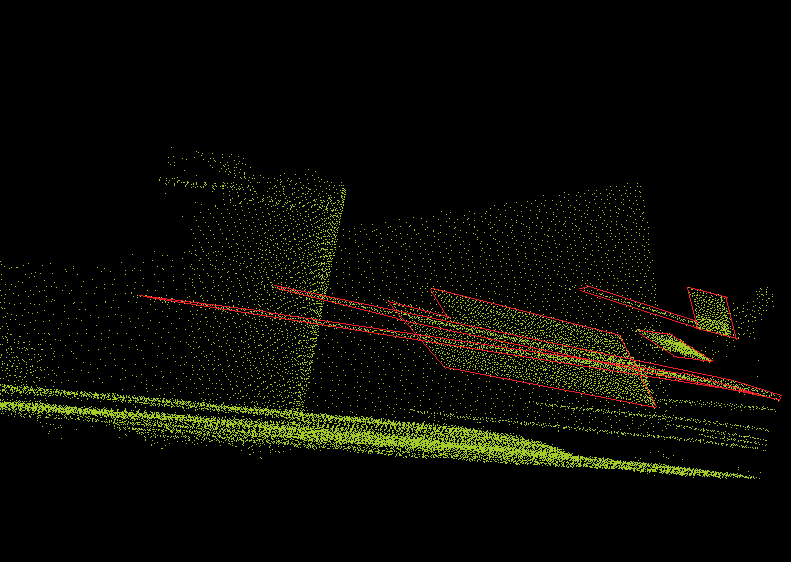
\includegraphics[width=0.9\columnwidth]{pointClouds/artefatti.png} 
    \caption{Point Cloud che presenta problemi di artefatti di un bidone conico, vista laterale}
    \label{figure:pcloud_artifacts}
\end{figure}

\subsection{Controllo di forma}
Oltre alla creazione del modello 3D e del calcolo del volume potrebbe rivelarsi molto utile per gli ispettori avere uno strumento automatico per confrontare la forma dell'oggetto ispezionato con un modello "pefetto" del bene stesso. Ad esempio potrebbe essere usato per confrontare componenti meccaniche con i loro modelli \emph{CAD} al fine di individuare eventuali deformazioni subite durante il trasporto.

%**************************************************************
\section{Consuntivo finale}

%**************************************************************
\section{Raggiungimento degli obiettivi}

%**************************************************************
\section{Conoscenze acquisite}

%**************************************************************
\section{Valutazione personale}
